\documentclass[11pt,aspectratio=43,usenames,dvipsnames]{beamer}
\usepackage[utf8]{inputenc}
\usepackage{amsmath, amsfonts, amssymb, amsthm}
\usepackage[T1]{fontenc}
% mint: code chuck and syntax highlighting
%% outputdir should change according to pdf build directory
\usepackage[outputdir=build,cache=false]{minted}
\usepackage{lmodern}
\usepackage{xcolor}
\usepackage{setspace}
\usepackage{booktabs}
\usepackage{multirow}
\usepackage{graphicx}
\usepackage[mode=tex]{standalone}

\usepackage{tikz}
\usetikzlibrary{decorations}
\usetikzlibrary{decorations.pathreplacing, intersections}
\usepackage{pgfplots}
\usetikzlibrary{calc,positioning}
\pgfplotsset{compat=newest, scale only axis, width = 10cm}
\pgfplotsset{sciclean/.style={axis lines=left,
        axis x line shift=0.5em,
        axis y line shift=0.5em,
        axis line style={-,very thin},
        axis background/.style={draw,ultra thin,gray},
        tick align=outside,
        xtick distance=1,
        ytick distance=1,
        major tick length=2pt}}

\usepackage{ulem}
\usepackage{hyperref}
\usepackage{booktabs}
\usepackage{babel}
\usepackage{makecell}
\usepackage[para,online,flushleft]{threeparttable}
\usepackage{pdfpages}
\usepackage{tcolorbox}
\usepackage{bm}
\usepackage{appendixnumberbeamer}
\usepackage{natbib}
\usepackage{caption}
\captionsetup[figure]{labelformat=empty}% redefines the caption setup of the figures environment in the beamer class.
\usetheme[compress]{Boadilla}
\usecolortheme{default}
\useoutertheme{miniframes}
\usefonttheme[onlymath]{serif}
\usepackage{fontawesome}

\newcommand{\jump}[2]{\hyperlink{#1}{\beamerbutton{#2}}}
\newcommand{\extjump}[2]{\href{#1}{\beamerbutton{#2}}}
\newcommand{\orange}[1]{\textcolor{orange}{#1}}
\newcommand{\red}[1]{\textcolor{red}{#1}}
\newcommand{\blue}[1]{\textcolor{blue}{#1}}
\newcommand{\green}[1]{\textcolor{OliveGreen}{#1}}

\renewcommand{\square}{\scalebox{0.7}{$\blacksquare$ \hspace{0.5em}}}
\setbeamertemplate{itemize item}{\raisebox{0.1em}{\scalebox{0.7}{$\blacksquare$}}}
\setbeamertemplate{itemize subitem}[circle]
\setbeamertemplate{itemize subsubitem}{--}
\setbeamercolor{itemize item}{fg=black}
\setbeamercolor{itemize subitem}{fg=black}
\setbeamercolor{itemize subsubitem}{fg=black}
\setbeamercolor{item projected}{bg=darkgray,fg=white}
\definecolor{blue}{rgb}{0.2, 0.2, 0.7}
\setbeamercolor{alerted text}{fg=blue}
\setbeamertemplate{enumerate items}[circle]


\setbeamertemplate{headline}{}

%==========================================
\let\olditemize=\itemize
\let\endolditemize=\enditemize
\renewenvironment{itemize}{\olditemize \itemsep1em}{\endolditemize}
\let\oldenumerate=\enumerate
\let\endoldenumerate=\endenumerate
\renewenvironment{enumerate}{\oldenumerate \itemsep1em}{ \endoldenumerate}

\DeclareMathOperator*{\argmax}{\arg\!\max}
\DeclareMathOperator*{\E}{\mathbb{E}}
\DeclareMathOperator*{\var}{\rm Var}
\DeclareMathOperator*{\cov}{\rm Cov}

\theoremstyle{definition}
\newtheorem{assume}{Assumption}
\newtheorem{lem}{Lemma}
\newtheorem{proposition}{Proposition}
\newtheorem{thm}{Theorem}
\newtheorem{corol}{Corollary}

\AtBeginSection[]{
  \begin{frame}[noframenumbering]
  \vfill
  \centering
  \begin{beamercolorbox}[sep=8pt,center,shadow=true,rounded=true]{title}
    \usebeamerfont{title}\insertsection\par%
  \end{beamercolorbox}
  \vfill
  \end{frame}
}

\begin{document}
    \title[Unit 6]{Unit 6 \\ The Firm: \\ Owners, Managers, and Employees}
    \author[Hui-Jun Chen]{Hui-Jun Chen}
    \institute[OSU]{The Ohio State University}
    % \date{\today}
    \date{\today}
    \setbeamertemplate{navigation symbols}{}
    \setstretch{1.2}

%-------------------------------------------------------
{
%	\usebackgroundtemplate{\includegraphics[width=1\paperwidth]{../EveningSky_cropped_edit43_bright.jpg}}
    \begin{frame}
% \vspace{3em}
        \centering
%		{\footnotesize 	ECON 4002 Intermediate Macroeconomic Theory}
        \maketitle
% \vspace{-1.5em}
% \centering
% \includegraphics[width=0.55\linewidth]{Pictures/houses.jpeg}


    \end{frame}
}

% -------------------------------------------
\setbeamertemplate{headline}
{
\setbeamercolor{section in head/foot}{fg=black, bg=white}
\vskip1em \tiny \insertsectionnavigationhorizontal{1\paperwidth}{\hspace{0.50\paperwidth}}{}
}
%------------------------------------------

\section[Intro]{Introduction}
\label{sec:Introduction}


\begin{frame}{Introduction}
\label{slide:Introduction}
    \begin{center}
        How does the firm interacts internally and externally?
    \end{center}
    \begin{itemize}
        \item Firms are legal entity, yet still are \alert{composed by human}
        \begin{itemize}
            \item internal: Owner(s) v.s. Managers
            \item external: Employees (labor market), consumer (goods market)
        \end{itemize}
        \item Internal conflict: asymmetric information (e.g. \cite{Akerlof_1970_TQJE})
        \item External conflict: hidden action (Principal-Agent Problem)
        \item As before, wage is determined by $ MRS = MRT $
        \item Further reading: \blue{\extjump{https://tinyurl.com/ysdzy8k9}{Unit 6}}
    \end{itemize}

\end{frame}

\section[Internal]{Internal Structure of the Firm}
\label{sec:Internal_Structure_of_the_Firm}

\begin{frame}{Firm's Internal Structure}
\label{slide:Firm_s_Internal_Structure}
    \begin{definition}
        Firm is a business organization which (1) hires ppl, (2) buy inputs to produce good/services, and (3) set prices $ \ge  $ cost.
    \end{definition}
    \begin{columns}
        \begin{column}{0.5\textwidth}
        \only<1> {Black arrow downward: }
        \only<2> {Green arrow upward: }
        \begin{itemize}
            \only<1> { \item Owners: set long-term goal }
            \only<1> { \item Managers: implement owners' goal by assigning tasks }
            \only<1> { \item Workers: doing tasks }
            \only<2> { \item Owners: Receive profit as a result of management}
            \only<2> { \item Managers: payment not directly related to effort $ \Rightarrow  $ other's \$, riskier investment / lowering effort }
            \only<2> { \item Workers: salary not increasing with effort}
        \end{itemize}
        \end{column}
        \begin{column}{0.5\textwidth}
            \begin{figure}
                \centering
                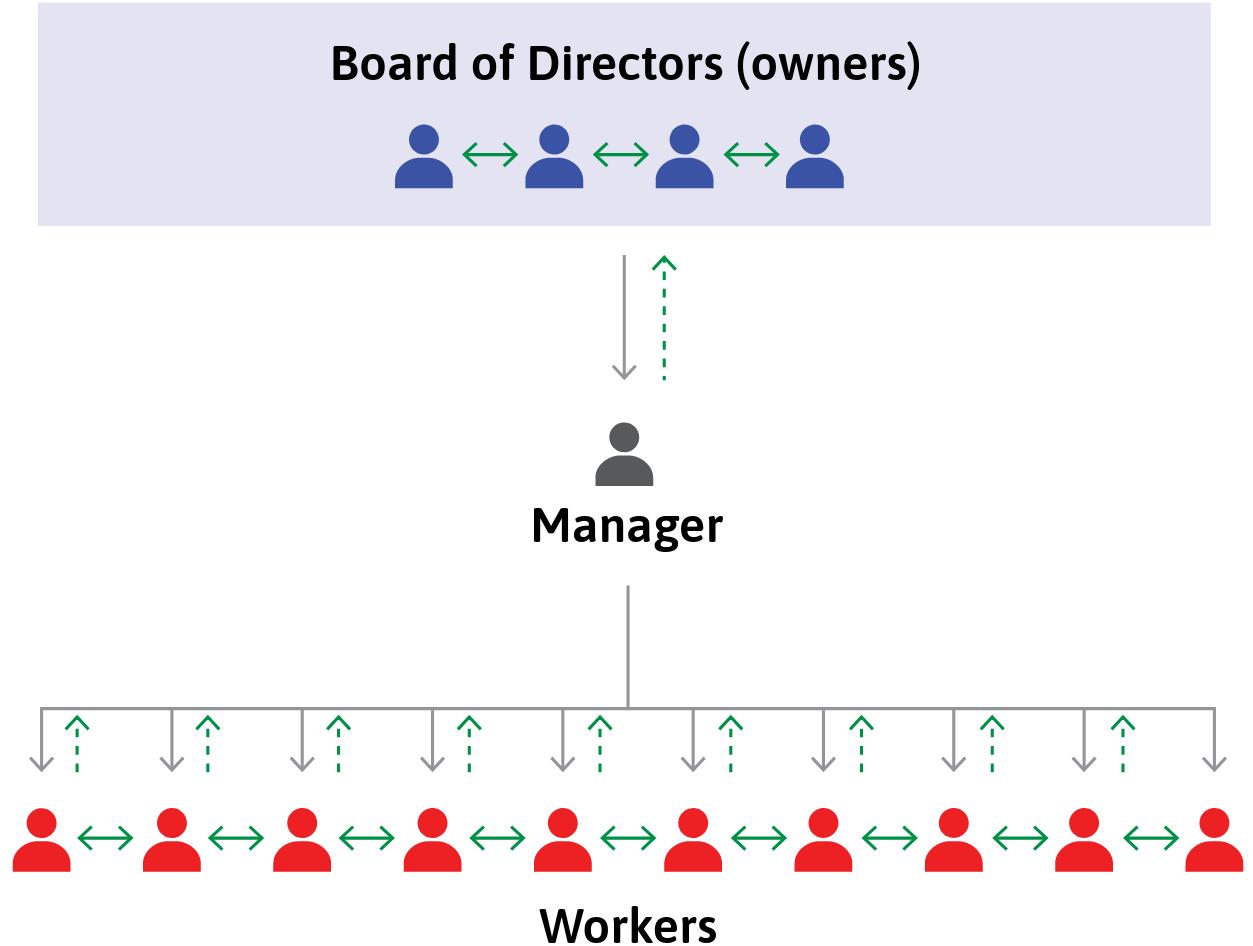
\includegraphics[width=\textwidth]{./figures/firmStructure.png}
            \end{figure}

        \end{column}
    \end{columns}

\end{frame}

\begin{frame}{Align the Interests}
\label{slide:Align_the_Interests}

    \begin{itemize}
        \item Contracts are \alert{incomplete}: outcome depends on \alert{future/unknown} events, and hard to \alert{measure} effort
        \item Incomplete contracts are inevitable, since modern job are mostly \textbf{not able to measure output} and \textbf{works as a team}
        \item Ways to alleviate incomplete contract:
        \begin{enumerate}
            \item pay with company shares: company profit $ \uparrow  $, share price $ \uparrow  $
            \item piece rate pay: \$5 to assembly one toy (low-end job)
            \item monitoring
        \end{enumerate}
    \end{itemize}
\end{frame}

\section[Labor]{Labor Discipline Model}
\label{sec:Labor_Discipline_Model}

\begin{frame}{Why do workers work hard?}
\label{slide:Why_do_workers_work_hard_}
    Workers work hard while firms' cannot directly measure effort because
    \begin{enumerate}
        \item work ethic
        \item feelings of responsibility
        \item reciprocate a feeling of gratitude for good working conditions
        \item benefits for measurable output
        \item promotions
        \item \alert{fear of being fired}
    \end{enumerate}
    \ldots Rational thinking sometimes means negative thinking \faMehO
\end{frame}

\begin{frame}{Fear of being Fired}
\label{slide:Fear_of_Fired}
    \begin{itemize}
        \item \alert{Rent} in Economics: payment to the owner greater than the costs
        \item If workers being unemployed, they get unemployment benefits $ \Rightarrow  $ \textbf{reservation wage}
        \item \alert{Employment rent}: benefit from employment $ - $ disutility from work $ - $ reservation wage, includes
        \begin{itemize}
            \item lost income when searching
            \item cost to start a new job, e.g. relocation
            \item Loss of non-wage benefits
            \item Social costs (scarring effects, lost of company connections/skill)
        \end{itemize}
        \item \alert{Larger employment rent (higher wage)} $ \Rightarrow  $ larger cost of job loss $ \Rightarrow  $ workers work hard to reduce chance of getting fired
    \end{itemize}
\end{frame}

\begin{frame}{Employment Game}
\label{slide:Employment_Game}
    \begin{enumerate}
        \item Employer: choose maximum wage to keep worker work hard enough
        \begin{itemize}
            \item payoff: output $ - $ wage
        \end{itemize}
        \item Worker: choose minimum effort to keep him/herself from firing
        \begin{itemize}
            \item payoff: employment rent
        \end{itemize}
        \item Workers are the \textbf{supply side} in labor market: trade off are \textbf{MRT}
        \item Employers are the \textbf{demand side} in labor market: trade off are \textbf{MRS}
        \item \alert{Best response curve}:
        \begin{itemize}
            \item for workers: optimal amount of effort workers will exert for each wage offered
            \item for employers: optimal level of wage employers will offer for each targeted level of effort.
        \end{itemize}
    \end{enumerate}
\end{frame}

\begin{frame}{Best response curves}
\label{slide:Best_response_curves}
    \begin{columns}
        \begin{column}{0.5\textwidth}
            Employers: \alert{assume revenue doesn't change}, firms minimize cost to max profit

            $ \Rightarrow  $ find a \textbf{isocost} line that minimize wage spending
            \begin{figure}
                \centering
                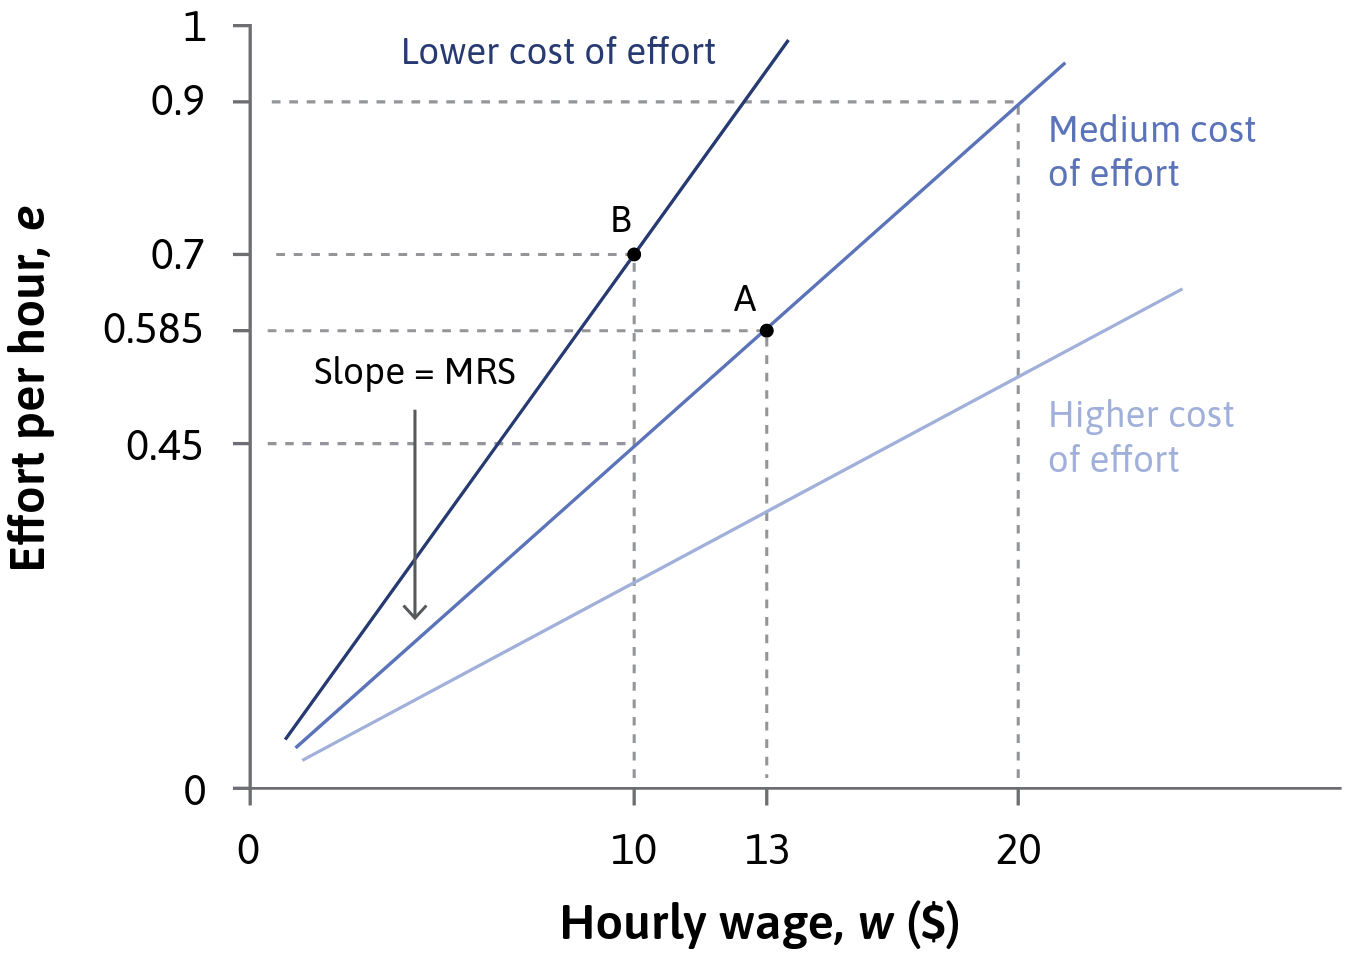
\includegraphics[width=\textwidth]{./figures/MRSEmployer.png}
            \end{figure}
        \end{column}
        \begin{column}{0.5\textwidth}
            Workers: Feasible frontier for wage \& effort
            \begin{figure}
                \centering
                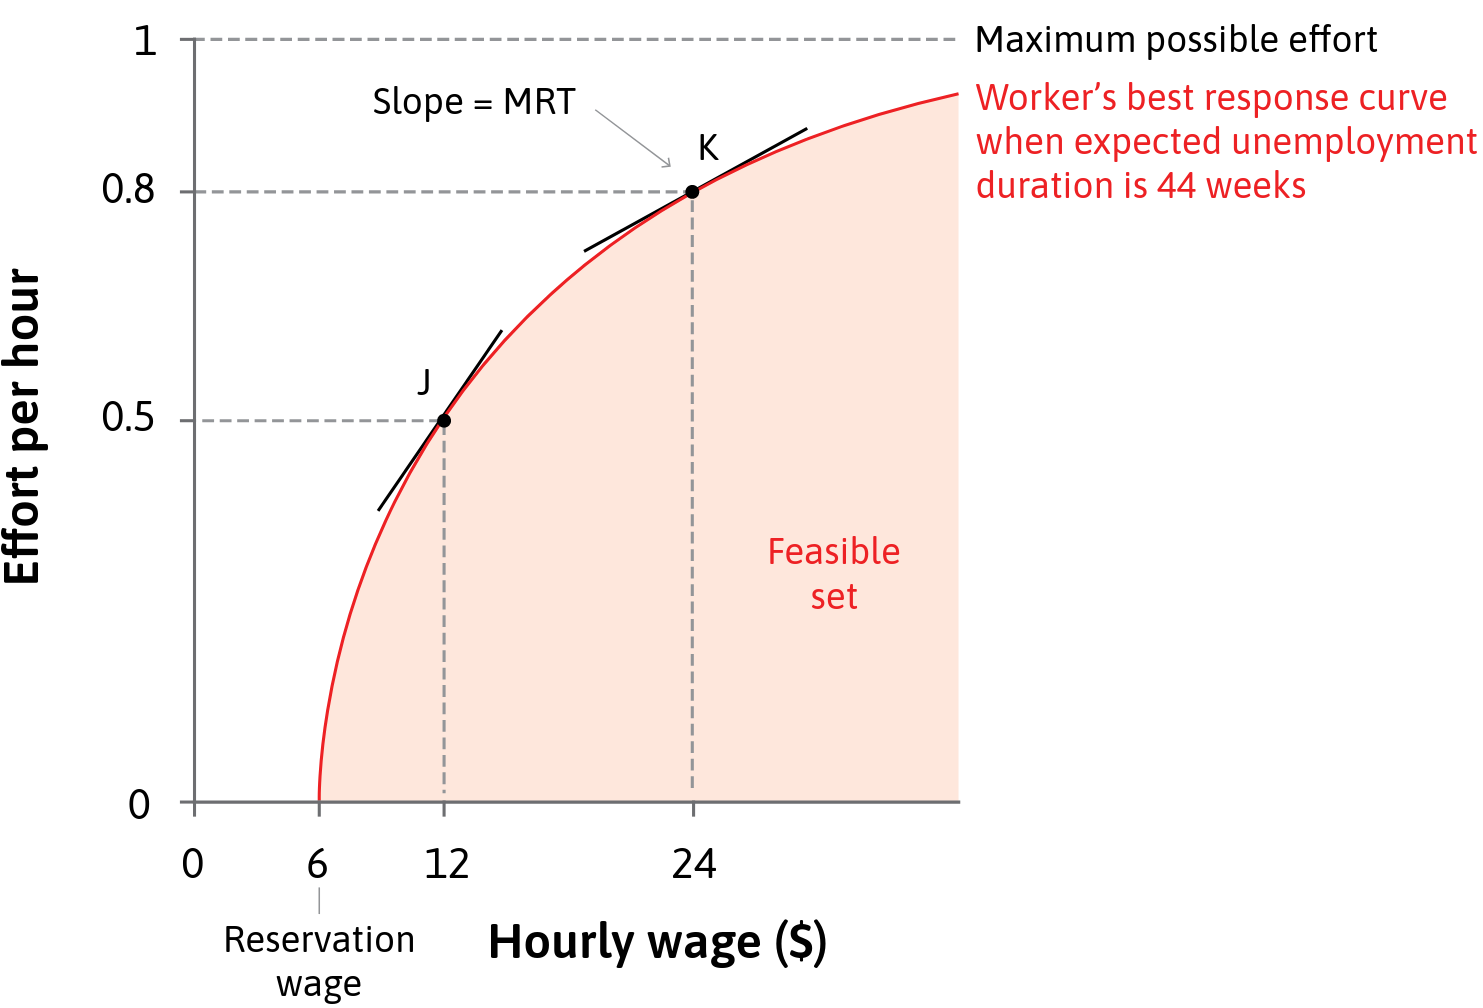
\includegraphics[width=\textwidth]{./figures/MRTWorkers.png}
            \end{figure}

        \end{column}
    \end{columns}

\end{frame}

\begin{frame}{Determining Wages}
\label{slide:Determining_Wages}
    Equilibrium is at MRS $ = $ MRT, efficiency wage $ = 12 >$ reservation wage
    \begin{figure}
        \centering
        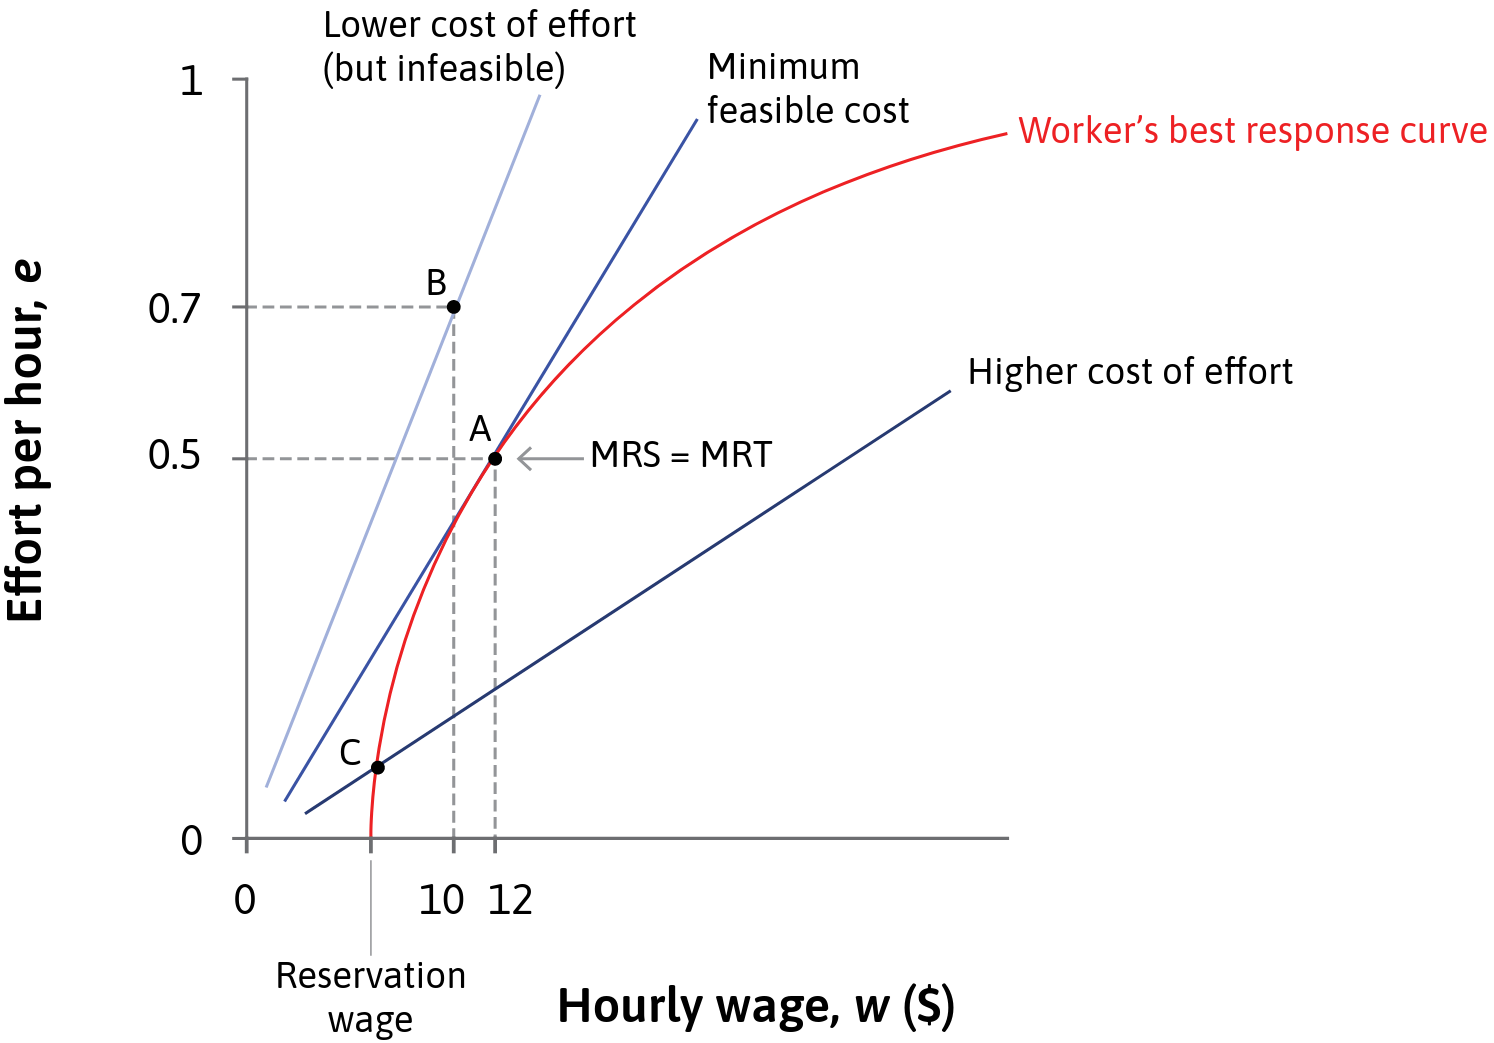
\includegraphics[width=0.8\textwidth]{./figures/EquilibriumLaborMkt.png}
    \end{figure}

\end{frame}

\begin{frame}{Involuntary Unemployment}
\label{slide:Involuntary_Unemployment}
    \begin{definition}
        \textbf{Involuntary unemployment} is being out of work, but preferring to have a job at the wages/working conditions as other workers.
    \end{definition}
    \begin{columns}
        \begin{column}{0.5\textwidth}
            \begin{itemize}
                \item Must have involuntary unemployment in the labor discipline model!
                \begin{itemize}
                    \item $ \because $ ensure employment rent is high enough for workers to put in effort.
                \end{itemize}
                \item Foreshadowing: How is unemployment rate $ \uparrow  $ affects the best response curve?
            \end{itemize}
        \end{column}
        \begin{column}{0.5\textwidth}
            \begin{figure}
                \centering
                \includestandalone[width=\linewidth]{./figures/BestResponse}
            \end{figure}
        \end{column}
    \end{columns}
\end{frame}

\section[P\&A]{Introduction for Principal-Agent Models}
\label{sec:Introduction_for_Principal_Agent_Models}

\begin{frame}{Incomplete Contracts in General}
\label{slide:Incomplete_Contracts_in_General}
    \begin{itemize}
        \item Incomplete contracts do not only occur in employment relationships.
        \item Incomplete contracts arise when:
        \begin{itemize}
            \item information is not verifiable
            \item the relationship covers periods of time
            \item there is uncertainty
            \item there are difficulties with measurement
            \item judiciary is absent
            \item preferences for omitting some information
        \end{itemize}

    \end{itemize}

\end{frame}

\begin{frame}{Principal-Agent models}
\label{slide:Principal_Agent_models}
    \begin{itemize}
        \item Principal-agent models capture interactions under incomplete contracts
        \begin{itemize}
            \item e.g. the firm is the principal and the worker is the agent
        \end{itemize}
        \item Agent takes action that is \alert{hidden} from the principal, which is why the principal cannot verify it.
        \begin{itemize}
            \item there is a conflict of interest between the principal and the agent
            \item over some action that may be taken by the agent
            \item and this action cannot be subjected to a complete contract.
        \end{itemize}
        \item The information about the action may be either asymmetric or unverifiable.
    \end{itemize}
\end{frame}


\section{Appendix}
\label{sec:Appendix}

\appendix
% -------------------------------------------
\setbeamertemplate{headline}
{
\setbeamercolor{section in head/foot}{fg=black, bg=white}
\vskip1em \tiny \insertsectionnavigationhorizontal{1\paperwidth}{\hspace{0.50\paperwidth}}{}
}
%------------------------------------------
% \begin{frame}\frametitle{}
% \begin{columns}
% \label{Appendix}
% \column{1\linewidth}
% \centering
% {\Large \alert{Appendix}}
% \end{columns}
% \end{frame}
%------------------------------------------
\begin{frame}[allowframebreaks]{References}
\footnotesize
\bibliographystyle{$BIB_STYLE}
\bibliography{$BIBFILE}
\end{frame}

\end{document}
